## Recursividad {.fragile}

\bgncolumns

\column{0.6\textwidth}

\vspace{-1em}

\bgnblockgood[wd=.8\textwidth,centered]
Maurits Cornelis Escher
\trmblockgood

\centering ``Drawing hands''

\column{0.4\textwidth}
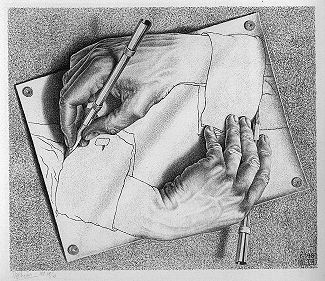
\includegraphics[width=0.8\textwidth,valign=t]{img/DrawingHands.jpg}
\trmcolumns

- Artista holandés.
- Célebre por sus obras inspiradas en temas relacionados con la matemática.
- Jugó impecablemente con figuras imposibles, desafiando las dimensiones espaciales.

- La paradoja en esta obra: ¿cuál es la mano que comenzó el dibujo?

## Recursividad {.fragile}

\simpleTitle{La base de la recursividad está en la naturaleza:}

¿Qué es un árbol?

- Un árbol es una rama.
- De una rama salen varias ramas.
- De una rama salen varias ramas.
- De una rama salen varias ramas.
- De una rama salen varias ramas.
...
- De una rama sale una hoja o una flor.

\bgnblocknormal
¿En qué se asemeja esto a un río?
\trmblocknormal

## Recursividad {.fragile}

\simpleTitle{Definamos entonces recursividad:}

\pause

\bgnblockdefinition
Para entender la \structure{recursividad},

\pause

primero hay que entender la \structure{recursividad}.

\trmblockdefinition

\bgncolumns

\column{.7\textwidth}

\only{<5>}{%

\footnotesize
\begin{itemize}
\item Para resolver su duda llame al 12345.
\item Usted ha llamado al 12345. Para contestar sus dudas, corte y marque el 12345.
\item Usted ha llamado al 12345. Para contestar sus dudas, corte y marque el 12345.
\item Usted ha llamado al 12345. Para contestar sus dudas, corte y marque el 12345.
\end{itemize}

}

\column{.3\textwidth}

\only{<4->}{%

\includegraphics[width=\textwidth,valign=t]{img/manthinking-1f914.pdf}
}

\trmcolumns

## Recursividad {.fragile}

\simpleTitle{Veamos una definición más amable:}

\bgnblockdefinition
\flushleft \vspace{-2ex} Un proceso es \structure{recursivo} si:
\vspace{1ex}

1. Tiene un caso base.
1. Hay una regla principal que se llama a sí misma
    - \normalsize \vspace{.4ex} Pero en cada llamado se va reduciendo.
    - Hasta finalmente llegar al caso base.

\vspace{.5ex}
\trmblockdefinition

\vfill

\bgncolumns
\column{.33\textwidth}
\centering

\includegraphics[width=.6\textwidth,valign=t]{img/spiral.png}
\column{.33\textwidth}
\centering

\includegraphics[width=.6\textwidth,valign=t]{img/samsung-shell.png}
\column{.33\textwidth}
\centering

\includegraphics[width=.6\textwidth,valign=t]{img/coffee_v10_2615.pdf}
\trmcolumns

## Recursividad {.fragile}

\simpleTitle{Ejemplos:}

- Elevar a potencias

$$ a^b = \begin{cases}
        1               & \;\;\;\;\text{si b = 0} \\
        a \cdot a^{b-1} & \;\;\;\;\text{si b > 0} \\
    \end{cases}
$$

- Factorial

$$ n! = \begin{cases}
        1               & \;\;\;\;\text{si n = 0} \\
        n \cdot (n-1)!  & \;\;\;\;\text{si n > 0} \\
    \end{cases}
$$

## Recursividad: aplicaciones {.fragile}

\bgnblockgood
\strongText{Ejemplo 1:} Imprimir una palabra $n$ veces.
\trmblockgood

\pause
\vspace{1ex}

\simpleTitle{Lo que sabemos hacer hasta ahora:}

\bgncolumns[-4ex]
\column{.6\textwidth}

- Imprimir la palabra 1 vez:

\column{.4\textwidth}

\begin{lstlisting}
def imprime(palabra):
    print(palabra)
\end{lstlisting}

\trmcolumns

\pause

\bgncolumns[-2ex]
\column{.6\textwidth}

- Para imprimirla 2 veces, podríamos hacer:

\column{.4\textwidth}

\begin{lstlisting}
(*@\tikzmark{markBgnBadCode}@*)def imprime2Veces(palabra):
    print(palabra)
    print(palabra)
\end{lstlisting}

\trmcolumns

\bgncolumns[-2ex]
\column{.6\textwidth}

- Para imprimirla 3 veces, podríamos hacer:

\column{.4\textwidth}

\begin{lstlisting}
def imprime3Veces(palabra):(*@\tikzmark{markMdlBadCode}@*)
    print(palabra)
    print(palabra)
    print(palabra)(*@\tikzmark{markTrmBadCode}@*)
\end{lstlisting}

\trmcolumns

\pause

\vspace{-2ex}
\bgnblockdanger
Esto último es muy mala idea: no es sustentable.
\trmblockdanger

\begin{tikzpicture}[remember picture, overlay]
  \node[fit=(pic cs:markBgnBadCode) (pic cs:markMdlBadCode) (pic cs:markTrmBadCode), inner sep=0em] (enc) {};
  \draw[red, line width=.4em, line cap=round] (enc.north west) -- (enc.south east);
  \draw[red, line width=.4em, line cap=round] (enc.north east) -- (enc.south west);
\end{tikzpicture}

## Recursividad: aplicaciones {.fragile}

\bgnblockgood
\strongText{Ejemplo 1:} Imprimir una palabra $n$ veces.
\trmblockgood

\simpleTitle[2ex]{¿Qué tal si aplicamos recursividad?}
\vspace{-1ex}

\pause

\bgncolumns
\column{.55\textwidth}

- \bld{Caso base}: $n = 0$
    - Se termina el programa.
- \bld{Caso recursivo}:
    - Imprime 1 vez la palabra.
    - Imprime $n-1$ veces la palabra.

\pause

\column{.45\textwidth}

\begin{lstlisting}[style=frame02]
# nVeces: str int -> None
# Imprime palabra n veces, cada
# una en su propia línea.
# Ejemplo: nVeces('playa', 7)
def nVeces(palabra, n):
    if n == 0:
        return
    else:
        print(palabra)
        nVeces(palabra, n - 1)
\end{lstlisting}

\trmcolumns

## Recursividad: aplicaciones {.fragile}

\bgnblockgood
\strongText{Ejemplo 2:} Imprimir una cuenta regresiva, desde $n$.
\trmblockgood

\vspace{1ex}

- Imprimir una cuenta regresiva:
    - Desde $n$ hasta 1.
    - Cuando toque el 0, imprimir un mensaje ad-hoc.

\bgncolumns
\column{.2\textwidth}
\column{.3\textwidth}

\pause
\ttt{4}\newline
\pause
\ttt{3}\newline
\pause
\ttt{2}\newline
\pause
\ttt{1}\newline
\pause
\ttt{¡A correr!}

\column{.3\textwidth}


\includegraphics[width=.9\textwidth]{img/racecar-1f3ce.pdf}

\column{.2\textwidth}
\trmcolumns

## Recursividad: aplicaciones {.fragile}

\bgnblockgood
\strongText{Ejemplo 2:} Imprimir una cuenta regresiva, desde $n$.
\trmblockgood

\simpleTitle[2ex]{¿Qué tal si aplicamos recursividad?}
\vspace{-1ex}

\pause

\bgncolumns[-1ex]
\column{.55\textwidth}

- \bld{Caso base}: llegamos a 0.
    - Imprimimos el mensaje.
    - Se termina el programa.
- \bld{Caso recursivo}:
    - Imprimir $n$.
    - Cuenta regresiva desde $n - 1$.

\column{.45\textwidth}

\begin{lstlisting}[style=frame02]
# cuentaRegresiva: int -> None
# Muestra una cuenta regresiva,
# desde n hasta 1. En vez del
# cero, presenta un mensaje.
# Ejemplo: cuentaRegresiva(8)
def cuentaRegresiva(n):
    if n == 0:
        print('¡A correr!')
        return
    else:
        print(n)
        cuentaRegresiva(n - 1)
\end{lstlisting}

\trmcolumns

## Recursividad: aplicaciones {.fragile}

\bgnblockgood
\strongText{Ejemplo 3:} Elevar a potencias.
\trmblockgood

$$ a^b = \begin{cases}
        1               & \;\;\;\;\text{si b = 0} \\
        a \cdot a^{b-1} & \;\;\;\;\text{si b > 0} \\
    \end{cases}
$$

\vspace{1ex}

- Por lo que para $b \in \mathbb{N}$:

\vspace{-1ex}
\begin{eqnarray*}
a^0 & = & 1 \\
a^1 & = & a \cdot a^0 \\
a^2 & = & a \cdot a^1 = a \cdot (a \cdot a^0) \\
a^3 & = & a \cdot a^2 = a \cdot (a \cdot a^1) = a \cdot (a \cdot (a \cdot a^0)) \\
    & \ldots & \\
a^n & = & a \cdot a^{n-1} = a \cdot (a \cdot a^{n-2}) = \ldots
\end{eqnarray*}


## Recursividad: aplicaciones {.fragile}

\simpleTitle{Elevar a potencias: ejemplo de desarrollo para \bld{a=2}, \bld{b=4}}

$$ a^b = \begin{cases}
        1               & \;\;\;\;\text{si b = 0} \\
        a \cdot a^{b-1} & \;\;\;\;\text{si b > 0} \\
    \end{cases}
$$

\vspace{-3ex}

\bgncolumns

\column{.6\textwidth}

\begin{footnotesize}
\begin{eqnarray*}
2^4 & = & 2 * 2^3 \tikzmark{bgnBraceReduction} \\
    & = & 2 * (2 * 2^2) \\
    & = & 2 * (2 * (2 * 2^1)) \\
    & = & 2 * (2 * (2 * (2 * 2^0)) \tikzmark{trmBraceReduction} \\
    & = & 2 * (2 * (2 * (2 * 1) \tikzmark{trmBraceBaseCase}) \\
    & = & 2 * (2 * (2 * 2)) \\
    & = & 2 * (2 * 4) \\
    & = & 2 * 8 \tikzmark{trmGathering} \\
2^4 & = & 16 \\
\end{eqnarray*}
\end{footnotesize}

\column{.3\textwidth}

\trmcolumns

\braceRightwardsLabel[text width=12em, brace/.style={xshift=.3em}]{bgnBraceReduction}{trmBraceReduction}{En cada paso se llama recursivamente a la misma función, pero reducida.\newline \newline }
\braceRightwardsLabel[brace/.style={xshift=1.3em}]{trmBraceReduction}{trmBraceBaseCase}{Llegamos al caso base.}
\braceRightwardsLabel[brace/.style={xshift=.3em}]{trmBraceBaseCase}{trmGathering}{\newline \newline Recolección de resultados de las llamadas recursivas.}
    

## Recursividad: aplicaciones {.fragile}

\bgncolumns
\column{.52\textwidth}
\bgnblockgood
\strongText{Ejemplo 3:} Elevar a potencias.
\trmblockgood

\column{.45\textwidth}
\vspace{-7ex}
$$ a^b = \begin{cases}
        1               & \;\;\;\;\text{si b = 0} \\
        a \cdot a^{b-1} & \;\;\;\;\text{si b > 0} \\
    \end{cases}
$$
\trmcolumns

\vspace{3ex}

\begin{lstlisting}[style=frame02]
# potencia: num int -> num
# Calcula el valor de base elevado a exp.
# Ejemplo: potencia(3, 4) retorna 81
def potencia(base, exp):
    if exp == 0:            # caso base
        return 1
    else:                   # caso recursivo
        return base * potencia(base, exp - 1)
# Tests
assert potencia(2, 7) == 128
assert potencia(-2, 3) == -8
assert potencia(1.5, 4) == 5.0625
\end{lstlisting}

## Recursividad: aplicaciones {.fragile}

\bgnblockgood
\strongText{Ejemplo 4:} Sumar los dígitos de un número.
\trmblockgood

\pause

\begin{lstlisting}[style=frame02]
# sumarDigitos: int -> int
# Calcula la suma de todos los dígitos que componen el
# número entregado como parámetro.
# Ejemplo: sumarDigitos(241) retorna 7
def sumarDigitos(numero):
    if numero == 0:            # caso base
        return 0
    else:                      # caso recursivo
        ultimo = numero % 10
        reducido = numero // 10
        return sumarDigitos(reducido) + ultimo
# Tests
assert sumarDigitos(64) == 10
assert sumarDigitos(9645) == 24
\end{lstlisting}


## Recursividad: aplicaciones {.fragile}

\bgnblockgood
\strongText{Ejemplo 5:} Obtener la cantidad de dígitos de un número.
\trmblockgood

\pause


\begin{lstlisting}[style=frame02]
# cantDigitos: int -> int
# Determina la cantidad de dígitos de un número.
# Ejemplo: cantDigitos(241) retorna 3
def cantDigitos(numero):
    if numero == 0:            # caso base
        return 0
    else:                      # caso recursivo
        reducido = numero // 10
        return 1 + cantDigitos(reducido)
# Tests
assert cantDigitos(64) == 2
assert cantDigitos(9645) == 4
\end{lstlisting}


## Recursividad: Conejitos cariñosos {.fragile}

\setbeamertemplate{itemize/enumerate body begin}{\footnotesize}
\setbeamertemplate{itemize/enumerate subbody begin}{\footnotesize}

\vspace{-2ex}

- Mes 0: De una casa se escapa una pareja de conejos bebés.
- Mes 1: Estos conejos, al mes ya son adultos.
- Mes 2: Ya tienen un par de crías.
    - Son de una raza que siempre paren un macho y una hembra.
- Mes 3: La pareja original tiene otro par de crías.
    - La primera pareja de hijos ya es adulta.
- Mes 4: La pareja original de nuevo tiene otro par de crías.
    - La primera pareja de hijos también aporta con un par de crías.
    - La segunda pareja de hijos ya es adulta.
- Mes 5: La pareja original de nuevo tiene otro par de crías.
    - La primera pareja de hijos tiene su segundo par de crías.
    - La segunda pareja de hijos pare por primera vez.
    - La tercera pareja de hijos ya es adulta.
- Así, sucesivamente...

\bgnblocknormal
¿Cuántas parejas de conejos hay en el mes \bld{n}?
\trmblocknormal

\placeLogo{img/rabbit-1f407.pdf}

## Recursividad: Conejitos cariñosos {.fragile}

\newcommand{\nzRbbS}{
\includegraphics[width=9mm]{img/twoRabbits.pdf}}
\newcommand{\nzRbbX}{
\includegraphics[width=12mm]{img/twoRabbits.pdf}}
\tikzset{
  % style for inserting images as nodes
  img/.style={
    % text width=8mm,
    minimum height=4mm,
    anchor=center,
    %text height=2cm,                 %% don't use this
    inner sep=0pt,     %% use this
    outer sep=0pt,     %% and this
    % rectangle,
    % align=center,
    % draw,thick % only for debugging..
  },
  treeLines/.style={
    ultra thick, black
  },
}
\begin{tikzpicture}

  \matrix (rbbs) [matrix of nodes, nodes=img, row sep=4mm, column sep=0mm]{
   \footnotesize{Mes}    &         &         &         &         &         &         &        &        & \footnotesize{Parejas} \\
   0 &         &         &         &         & \nzRbbS &         &         &         & 1      \\
   1 &         &         &         &         & \nzRbbX &         &         &         & 1      \\
   2 &         & \nzRbbS &         &         & \nzRbbX &         &         &         & 2      \\
   3 &         & \nzRbbX &         &         & \nzRbbX &         & \nzRbbS &         & 3      \\
   4 & \nzRbbS & \nzRbbX &         & \nzRbbS & \nzRbbX &         & \nzRbbX &         & 5      \\
   5 & \nzRbbX & \nzRbbX & \nzRbbS & \nzRbbX & \nzRbbX & \nzRbbS & \nzRbbX & \nzRbbS & 8      \\
  };

% parejas
\draw[treeLines] (rbbs-2-6) -- (rbbs-3-6);
\draw[treeLines] (rbbs-3-6) -- (rbbs-4-6);
\draw[treeLines] (rbbs-4-6) -- (rbbs-5-6);
\draw[treeLines] (rbbs-5-6) -- (rbbs-6-6);
\draw[treeLines] (rbbs-6-6) -- (rbbs-7-6);
% parejas
\draw[treeLines] (rbbs-4-3) -- (rbbs-5-3);
\draw[treeLines] (rbbs-5-3) -- (rbbs-6-3);
\draw[treeLines] (rbbs-6-3) -- (rbbs-7-3);
% parejas
\draw[treeLines] (rbbs-5-8) -- (rbbs-6-8);
\draw[treeLines] (rbbs-6-8) -- (rbbs-7-8);
% parejas
\draw[treeLines] (rbbs-6-2) -- (rbbs-7-2);
% parejas
\draw[treeLines] (rbbs-6-5) -- (rbbs-7-5);

% hijos
\draw[treeLines] (rbbs-3-6) -- (rbbs-4-3);
\draw[treeLines] (rbbs-4-6) -- (rbbs-5-8);
\draw[treeLines] (rbbs-5-3) -- (rbbs-6-2);
\draw[treeLines] (rbbs-5-6) -- (rbbs-6-5);
\draw[treeLines] (rbbs-6-3) -- (rbbs-7-4);
\draw[treeLines] (rbbs-6-6) -- (rbbs-7-7);
\draw[treeLines] (rbbs-6-8) -- (rbbs-7-9);

\end{tikzpicture}

## Recursividad: Sucesión de Fibonacci {.fragile}

\bgnblocknormal
\bld{La sucesión de Fibonacci} se define recursivamente como:
\trmblocknormal

\vspace{-2ex}

$$ F_n = \begin{cases}
        n                 & \;\;\;\;\text{si} \;\;\;\; 0 \leq n \leq 1 \\
        F_{n-1} + F_{n-2} & \;\;\;\;\text{si} \;\;\;\; n > 1 \\
    \end{cases}
$$

\vspace{1ex}
\begin{lstlisting}[style=frame02]
# fibonacci: int -> int
# Calcula el n-ésimo valor de la sucesión de Fibonacci.
# Ejemplo: fibonacci(8) retorna 21
def fibonacci(n):
    if n <= 1:            # caso base
        return n
    else:                 # caso recursivo
        return fibonacci(n - 1) + fibonacci(n - 2)
# Tests
assert fibonacci(0) == 0
assert fibonacci(9) == 34
\end{lstlisting}

## Recursividad: Sucesión de Fibonacci {.fragile}

\simpleTitle{La espiral de Fibonacci:}

\bgncolumns
\column{.45\textwidth}

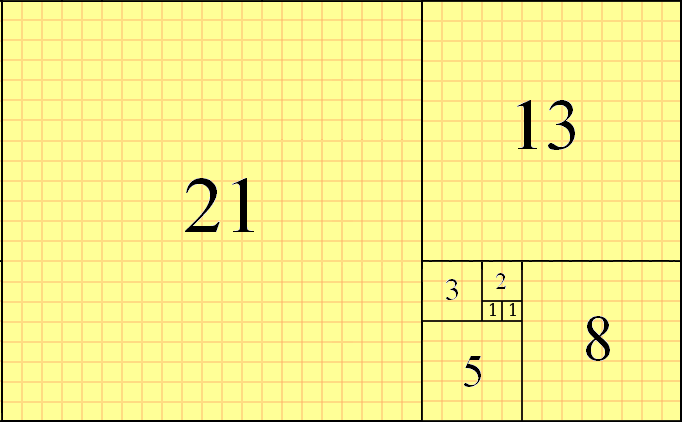
\includegraphics[width=\textwidth]{img/FibonacciBlocks.png}

\scriptsize{https://commons.wikimedia.org/
wiki/File:34*21-FibonacciBlocks.png}
\column{.1\textwidth}
\column{.45\textwidth}


\includegraphics[width=\textwidth]{img/fibonacci-nature-3.jpg}

\scriptsize{iStockphoto.com/Janne Ahvo}

\trmcolumns
